\chapter{Emocje w grach}
\label{chap:trzeci}

\section{Wprowadzenie}

Grę komputerową definiujemy jako cyfrowe interaktywne doświadczenie dla jednego bądź wielu graczy. Od czasów powstania pierwszej gry wideo, to medium przeszło zauważalną transformację. W dzisiejszych czasach istnieje szeroki wachlarz typów gier wideo - od napiętego, filmowego doświadczenia pojedynczego gracza przedstawionego na rysunku \ref{fig:cod} (seria Call of Duty), po relaksujące doświadczenia wymagające cierpliwości (FarmVille) ukazane na rysunku \ref{fig:farm}. Gry wideo to ewoluujące medium, a ich potencjał wciąż jest badany. Toczą się gorące dyskusje na temat tego, czy gry można zaklasyfikować jako sztukę, czy nie. Słownik oksfordzki opisuje grę jako dzieło, które należy docenić przede wszystkim za piękno lub siłę emocjonalną \citep{button}.


\begin{figure}[ht]
    \centering
    \begin{minipage}{0.45\textwidth}
        \centering
        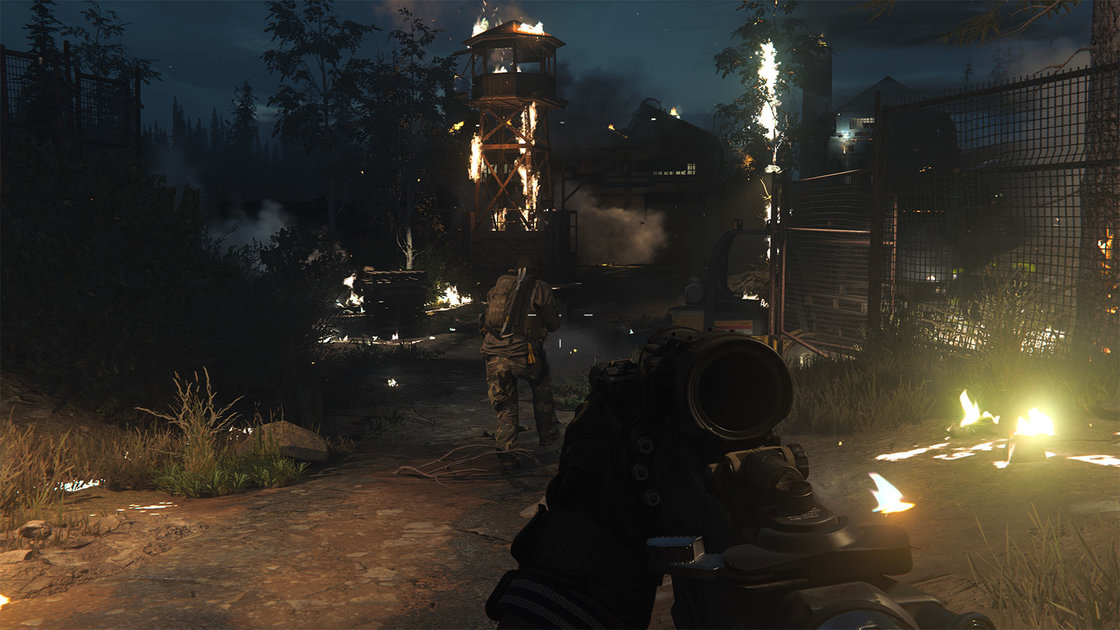
\includegraphics[width=1\textwidth]{images/cod.jpg} % first figure itself
        \caption{Widok z perspektywy pierwszej osoby z gry Call of Duty.}
        \caption*{Źródło: https://www.pocket-lint.com /games/reviews/activision/150364-call-of-duty-modern-warfare-review}
        \caption*{Data dostępu: 12.05.2020}
        \label{fig:cod}
    \end{minipage}\hfill
    \begin{minipage}{0.45\textwidth}
        \centering
        
\includegraphics[width=1\textwidth]{images/farm.jpg} % second figure itself
        \caption{Widok gracza wraz z interfejsem użytkownika z gry FarmVille.}
        \caption*{Źródło: https://www.pocketgamer.com /games/023284/farmville-2-country-escape/screenshots/}
        \caption*{Data dostępu: 12.05.2020}
        \label{fig:farm}
    \end{minipage}
\end{figure}

Twórcy gier z reguły kopiują metody wywołania emocji z uznanych już wcześniej mediów - literatury i filmu. Gracze grają w gry dla doświadczenia pewnego przeżycia, a gry mają zdolność symulowania emocji w formie bliższej prawdziwemu życiu niż filmy czy książki. Mając to na uwadze, gry powinny mieć potencjał wywoływania silnych emocji, w połączeniu z konwencjonalnymi sposobami wykorzystanymi w wyżej wymienionych mediach, ale również bez ich wykorzystania. Jeśli chodzi o wywołanie emocji, potencjał gier wydaje się większy \citep{button, movesus}.

\section{Wymiary emocji}

Teorie emocji mówią, że ludzie są ewolucyjnie wyposażeni w ograniczony zestaw podstawowych emocji. Każda podstawowa emocja jest niezależna od innych w jej behawioralnych (związanych z zachowaniem), psychologicznych i fizjologicznych przejawach. Wyróżnia się sześć podstawowych emocji, a mianowicie \citep{colors}:
\begin{itemize}
  \item gniew,
  \item strach,
  \item wstręt,
  \item radość,
  \item smutek,
  \item zaskoczenie.
\end{itemize}

Większość teoretyków podziela pogląd, że emocje składają się z trzech głównych elementów: subiektywnego odczuwania, ekspresji i reakcji fizjologicznej. Jedne są motywacyjne i mają tendencję do wprowadzenia w stan motywacyjny lub tendencję do działania \citep{games}.

Istnieje możliwość określenia emocji, badając mimikę i reakcje fizjologiczne. Emocje można mierzyć również pośrednio za pomocą reakcji emocjonalnych. Badania pozwoliły na stworzenie modelu reakcji emocjonalnych.  Wymiarowa teoria emocji utrzymuje, że wszystkie emocje mogą znajdować się w dwuwymiarowej przestrzeni, jako współrzędne walencji oraz pobudzenia \citep{games}.

Jednym z często używanych modeli jest „kołowy model afektu” stworzony przez Russella w 1980 roku, który został przedstawiony na rysunku \ref{fig:spectrum}. Charakteryzuje on emocje w kategoriach dwóch wymiarów reakcji emocjonalnych, a mianowicie pobudzenia i walencji. Pobudzenie to fizjologiczny i psychologiczny stan bycia pobudzonym (aktywacja) lub brakiem pobudzenia (dezaktywacja) na bodźce. Walencja jest wewnętrznie pozytywnym (przyjemnym) lub negatywnym (nieprzyjemnym) uczuciem, które jest wywołane przez wydarzenie, przedmiot lub sytuację \citep{colors}.

\begin{figure}[h]
	\centering
	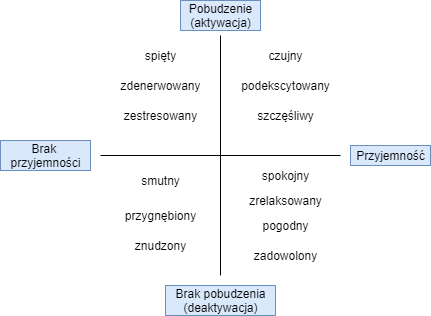
\includegraphics[width=0.85\textwidth]{images/diagram2.png}
	\caption{Kołowy model afektu stworzony przez Jamesa Russella. Oś pozioma odpowiada za walencję, a pionowa za stan pobudzenia.}
	\caption*{Źródło: opracowanie własne na podstawie \citep[s.1]{colors}.}
	\label{fig:spectrum}
\end{figure}


\section{Emocjonalne reakcje graczy}

Istnieje niewiele badań analizujących reakcje emocjonalne na gry z punktu widzenia doświadczenia użytkownika. Jednak niektóre badania dotyczyły jedynie negatywnie ocenianych emocji wywoływanych przez gry wideo, próbując rozwikłać ich potencjalne niekorzystne skutki. Badania były sprzeczne - jedne stwierdzały, że brutalne gry wideo wywołują wrogi afekt np. lęk, inne z kolei, że nie wywołują żadnego afektu. Ewentualnie niepokój może wynikać z obserwacji poziomu symbolicznej agresji, jaką samemu dokonuje się w grze. W odniesieniu do fizjologicznego komponentu emocji powszechnie wiadomo, że zadania wymagające wysiłku poznawczego lub aktywnego radzenia sobie wywołują pobudzenie emocjonalne, któremu towarzyszy m.in. przyspieszenie tętna. W badaniach nad psychofizjologiczną reaktywnością na stres, gry wideo były często wykorzystywane jako stresor. Kilka badań wykazało, że różne gry wideo wywołują znaczną reaktywność sercowo-naczyniową. Odkryto również, że dwuosobowa gra wideo na przykładzie „piłki nożnej” ma większy wpływ na tętno w porównaniu z grą wideo „trening squasha” przeciwko maszynie, co może sugerować, że sytuacja konkurencji społecznej związana z poprzednią grą powoduje zwiększone pobudzenie \citep{games}.


\section{Narzędzia wykorzystywane do wywołania emocji w grach}

\subsection{Awatar}

Awatar to byt, który wywodzi się z hinduskiej koncepcji boga wcielonego w różne istoty. Cyfrowy awatar to postać w wirtualnym świecie, która reprezentuje gracza. Bywają z góry zdefiniowane (tak jak postacie filmowe) lub istnieje możliwość  modyfikacji ich różnych cech: wyglądu, charakteru lub poziomu umiejętności \citep{glossary}.

Awatar jest często używany jako sposób na przeniesienie gracza do świata gry. Awatarów może być kilka i można ich używać na różne sposoby, ale łączy je to, że służą jako przedłużenie tożsamości gracza. Percepcja może wykroczyć poza świat realny, przenikając do wirtualnego i to samo dzieje się z tożsamością. Można to przyrównać do jazdy samochodem, kiedy podczas jazdy kierowca wyczuwa pozycje samochodu w przestrzeni, a ściślej określając do tzw. intuicyjnego ``wyczucia samochodu'' na przykład podczas parkowania - wtedy samochód staje się przedłużeniem ciała i jaźni \citep{gamefeel}.

Przedłużenie zmysłów gracza poprzez wcielenie się w postać pozwala zatracić się użytkownikowi w świecie gry. Daje to twórcom możliwość wywołanie różnych emocji u gracza, które odczuwa postać, w zależności od wydarzeń, które miały miejsce w symulowanym świecie. Zdarzenia występujące w grze np. walka postaci z lwem, może wywołać różne stany emocjonalne u różnych graczy - jedni poczują strach i wycofanie przed trudnym przeciwnikiem, inni z kolei będą pobudzeni i podekscytowani - gotowi na stoczenie walki. Tak więc mechanizm wywołania emocji w grze może być diametralnie inny od tego, który spotykamy w filmach, gdzie odczuwanie emocji jest zdeterminowane przez bierną obserwację poczynań bohaterów oraz ich przeżyć emocjonalnych. Emocje wywołane przez gry są zatem bardziej osobiste, ale trudniej je kontrolować twórcom. Składa się to na doświadczenie, będące dużo bardziej realne niż to filmowe \citep{button}.

\subsection{Interaktywność}

Interaktywność w kontekście gier, to termin, który jest używany do opisania jak gracz doświadcza historii, mechaniki i środowiska gry. Pozwala na zainteresowanie i zaangażowanie gracza. Podstawą tworzenia gier i główną cechą, która odróżnia gry od filmów jest interaktywność, co pozwala na nazwanie czynności grania aktywnym użyciem medium. W przeciwieństwie do pasywnych użyć mediów, aktywne ich użycie zmienia reakcje organizmu - zwiększa czujność poznawczą, tak więc granie w godzinach wieczornych może doprowadzić do wydłużenia czasu, który jest potrzebny na przejście z czasu czuwania do pełnego snu. Większość gier może być trudna do skończenia bez odpowiednich umiejętności i obycia ze sprzętem - tak więc gry wymagają od gracza uwagi i mocnego zaangażowania w to co się dzieje co może być dodatkowo bardzo skutecznie wykorzystane do wywołania emocji \citep{button, website:interactive}.

\subsection{Kontrola}

Kluczem do przeniesienia tożsamości gracza do świata gry jest kontrola w czasie rzeczywistym- czyli sterowanie poczynaniami awatara. Sterować można postaciami jak i bytami abstrakcyjnymi. Gry oparte na systemie turowym, lub takie, w których gracz nie wciela się w postać w pierwszej osobie, lecz sprawuje kontrolę pośrednio wydając rozkazy utrudniają identyfikację gracza z awatarem \citep{button}.

Urządzenia wejścia również przekładają się na satysfakcję gracza. Bardziej naturalne sposoby kontroli pozwalają na mocniejsze zatracenie się w grze. Użycie akcesoriów jak np. kierownica do grania w gry typu wyścigi, dostarczy graczowi dużo większych emocji niż kierowanie wirtualnym samochodem przy użyciu klawiatury \citep{button}.

Przeniesieniu tożsamości na awatar, pozwala graczowi na przeżycie tego co dzieje się na monitorze personalnie. Stąd też podczas animowanych przerywników filmowych w grach, gracz utożsamiający się z postacią przeżyje wydarzenia, które dzieją się na ekranie w sposób emocjonalny \citep{button, gamefeel}.

\subsection{Poczucie sprawczości}

Poczucie sprawczości występuje kiedy gracz bierze czynny udział w powieści i ma wpływ na jej przyszłe losy. W momentach, kiedy gracz tego doświadcza nie skupia się on na tym co aktualnie dzieje się w historii, natomiast na tym co stanie się w przyszłości, jeśli jakieś konkretne działania zostaną przez niego podjęte. Dzięki temu gracz czuje się odpowiedzialny, za to co dzieje się w fabule, nawet jeśli jego wpływ na nią jest bardzo mały. Taka zmiana pozwala na mocniejsze zaangażowanie i łatwiejsze wywołanie u niego konkretnych stanów emocjonalnych \citep{button, glossary}. 

Doświadczenie sprawczości to unikalne narzędzie wykorzystywane przez twórców gier. Poprzez dobrze zaprojektowane doświadczenie, gracz poczuje się odpowiedzialny za znacznie więcej niż w rzeczywistości, przy jednoczesnej oszczędności zasobów na zbyt szeroką i rozgałęzioną ścieżkę  \citep{button}.

\subsection{Symulowane akcje}

Symulowane akcje w kontekście gier występuje wtedy, kiedy interaktywność w grze wykracza poza korzystanie z funkcji interfejsu użytkownika. Elementy sterujące w grze mogą być zaprojektowane w sposób, który wywołuje emocje, jeśli tylko są one połączone z odpowiednią akcją. Dzieje się to najczęściej poprzez naśladowanie przez te elementy obiektów fizycznych. Jednym z przykładów symulowanej akcji może być proces przebiegu czasu. Ten wygenerowany przez świat gry wywołuje silne emocje, kiedy to na przykład pewne zadania muszą zostać rozwiązane w ograniczeniu czasowym - podobnie jak w sytuacjach generujących emocje w prawdziwym życiu. W takim przypadku gracz musi szybko zintegrować: procesy poznawcze, emocje oraz akcje w celu odniesienia sukcesu \citep{button}.

Kolejnym przykładem jest naśladowanie obiektów lub akcji występujących w grze przez kontrolery, które służą do sterowania. Niektóre są zbudowane tylko w celu imitacji danego elementu takie jak na przykład kierownice do samochodów lub drążki do latania. Pozwalają one na wywołanie silniejszych i bardziej realnych przeżyć u gracza, ale są za to mniej uniwersalne od klasycznych kontrolerów \citep{button}.

\subsection{Interaktywny dyskomfort}

Gry wideo nie zawsze muszą być zabawą i sprawiać radość. Podobnie jak inne media, mogą wywoływać różne rodzaje emocji i doświadczeń. Dyskomfort można wywołać na wiele różnych sposobów i chociaż może wydawać się to negatywnym zjawiskiem, może być odbierane pozytywnie. Zależy to od kontekstu - wiele graczy gra w gry wyłącznie dla negatywnie nacechowanych emocji np. strachu w grach typu horror \citep{button}.

Na podstawie badań J.A. Bopp negatywne emocje wywołane w grach mogą prowadzić do pozytywnych doświadczeń. Gracze oceniają gry nie tylko, ze względu na wywoływanie konkretnie nacechowanych emocji, ale także ze względu na fakt, że gra wywołuje silne reakcje emocjonalne, np. strach \citep{negativeemotions}.

% Na podstawie badań J.A. Bopp negatywne emocje wywołane w grach mogą prowadzić do pozytywnych doświadczeń. Gracze oceniają gry nie tylko, ze względu na wywoływanie konkretnie nacechowanych emocji, ale także, ze względu na wywołanie silnych reakcji emocjonalnych. 

% także ze względu na fakt, że gra wywołuje silne reakcje emocjonalne, np. strach \citep{negativeemotions}.


\subsection{Wyzwanie}

Wyzwanie to integralna część większości gier komputerowych występująca w różnorakiej formie. Głównymi czynnikami decydującymi o wyzwaniu są umiejętności gracza: czas reakcji, umiejętność prowadzenia wielu zadań na raz (tzw. multitasking) czy wysoki poziom opanowania kontrolera. Założenie określonego poziomu umiejętności dla wszystkich potencjalnych graczy jest niemożliwe, ale jeśli wyzwanie jest na odpowiednim poziomie dla konkretnego gracza, może on wejść w stan przepływu (ang. flow). Określa to tzw. Teoria Przepływu, którą Swink opisuje następująco: 
``Teoria przepływu mówi, że kiedy wyzwanie, które podejmujesz jest bardzo bliskie twojemu obecnemu poziomowi umiejętności, wejdziesz w stan ``flow'', który charakteryzuje się utratą samoświadomości,  zniekształconym postrzeganiem czasu i mnóstwem przyjemnych wrażeń. Jeśli twoje umiejętności są znacznie większe niż wyzwanie jakie daje Ci dana czynność, będziesz się nudzić, a jeśli twoje umiejętności są znacznie poniżej poziomu przewidzianego wyzwania będziesz sfrustrowany'' \citep[s.~23]{gamefeel}. Wyzwanie często jest używane aby wprowadzić gracza w stan ``flow'', co również  również potęguje jego emocje wynikające z rozgrywki \citep{button, gamefeel}.

\subsection{Doświadczenie społeczne - rozgrywka wieloosobowa}

W grach wieloosobowych działania każdej postaci z osobna łączą się tworząc jedno, społeczne doświadczenie pomiędzy graczami. Pomimo tego, że gracz nie znajduje się w realnym, lecz w ``wirtualnym świecie'', wykorzystuje się narzędzia, które pozwalają zaangażować się w społeczne odgrywanie ról przez awatary. Hybrydowy charakter tych doświadczeń, które są zarazem realne i wirtualne, pozwala na większe zaangażowanie graczy, którzy wcielają się w wykreowane postacie. W efekcie to projektanci gier kształtują środowisko społeczne oraz to w jaki sposób budowane są więzi społeczne między wieloma graczami, poprzez definicje sposobu interakcji między nimi \citep{movesus}.

\subsection{Zaangażowanie ciała}

Ciało znacząco kształtuje doświadczenie emocjonalne - tak samo w rozgrywce jak i w prawdziwym życiu. Od pojawienia się kontrolerów i urządzeń opartych na ruchu, twórcy gier mogą pozwolić na wykorzystanie ciała graczy jako medium do kształtowania emocji, bądź więzi społecznych. Projektanci gier wprowadzają coraz to bardziej innowacyjne rozwiązania, które pozwalają na wywołanie szerokiej palety emocji poprzez łączenie technologii, świata rzeczywistego i wyobraźni. Dzieje się tak na przykład poprzez zastosowanie strategii wymagających od graczy opanowania zmęczenia i bólu lub ułożenia ciała w sposób, który wywołuje fizyczną bliskość lub wymaga wyjścia ze strefy komfortu. Zamiast unieruchamiać ciało lub izolować graczy od innych ludzi, gry w przyszłości mogą obejmować i wzmacniać rolę ciała i jego fizycznej aktywności w grze. Połączenie fizyczne i emocjonalne może wspierać ludzi w dążeniu do osiągnięcia określonych efektów jak na przykład wytrenowanie wymarzonej sylwetki \citep{movesus}.